%%%%%%%%%%%%%%%%%%%%%%%%%%%%%%%%%%%%%%%%%%  不使用 authblk 包制作标题  %%%%%%%%%%%%%%%%%%%%%%%%%%%%%%%%%%%%%%%%%%%%%%
%-------------------------------PPT Title-------------------------------------
\title{材料智能计算业务介绍}
%-----------------------------------------------------------------------------

%----------------------------Author & Date------------------------------------
\author[\textrm{Jun\_Jiang}]{姜\;\;骏\inst{}} %[]{} (optional, use only with lots of authors)
%% - Give the names in the same order as the appear in the paper.
%% - Use the \inst{?} command only if the authors have different
%%   affiliation.
\institute[BCC]{\inst{}%
%\institute[Gain~Strong]{\inst{}%
\vskip 2pt %北京市计算中心}
云平台事业部~材料计算团队}
%\vskip -20pt {\large 格致斯创~科技}}
\date[\today] % (optional, should be abbreviation of conference name)
{	%{\fontsize{6.2pt}{4.2pt}\selectfont{\textcolor{blue}{E-mail:~}\url{jiangjun@bcc.ac.cn}}}
\vskip 20 pt {\fontsize{8.2pt}{6.2pt}\selectfont{%清华大学\;\;物理系% 报告地点
	\vskip 5 pt \textrm{2024.05.17}}}
}

%% - Either use conference name or its abbreviation
%% - Not really information to the audience, more for people (including
%%   yourself) who are reading the slides onlin%%   yourself) who are reading the slides onlin%%   yourself) who are reading the slides onlineee
%%%%%%%%%%%%%%%%%%%%%%%%%%%%%%%%%%%%%%%%%%%%%%%%%%%%%%%%%%%%%%%%%%%%%%%%%%%%%%%%%%%%%%%%%%%%%%%%%%%%%%%%%%%%%%%%%%%%%

\subject{}
% This is only inserted into the PDF information catalog. Can be left
% out.
%\maketitle
\frame
{
%	\frametitle{\fontsize{9.5pt}{5.2pt}\selectfont{\textcolor{orange}{“大数据中心调研座谈会”}}}
\titlepage
}
%-----------------------------------------------------------------------------

%------------------------------------------------------------------------------列出全文 outline ---------------------------------------------------------------------------------
%\section*{}
%\frame[allowframebreaks]
%{
%  \frametitle{Outline}
%%  \frametitle{\textcolor{mycolor}{\secname}}
%  \tableofcontents%[current,currentsection,currentsubsection]
%}
%%在每个section之前列出全部Outline
%%类似的在每个subsection之前列出全部Outline是\AtBeginSubsection[]
%\AtBeginSection[]
%{
%  \frame<handout:0>%[allowframebreaks]
%  {
%    \frametitle{Outline}
%%全部Outline中,本部分加亮
%    \tableofcontents[current,currentsection]
%  }
%}

%-----------------------------------------------PPT main Body------------------------------------------------------------------------------------
\small
\begin{frame}{科学研究的重要助手:~计算模拟}
\begin{figure}[h!]
\vspace*{-0.18in}
\centering
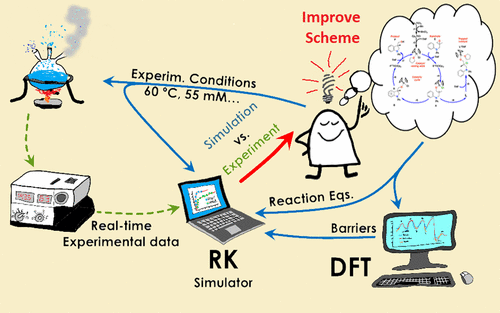
\includegraphics[height=2.55in,width=4.05in]{Figures/Schematic_Material-Design.png}
%\caption{\tiny \textrm{Pseudopotential for metallic sodium, based on the empty core model and screened by the Thomas-Fermi dielectric function.}}%(与文献\cite{EPJB33-47_2003}图1对比)
%\caption{\tiny \textrm{Pseudopotential for metallic sodium, based on the empty core model and screened by the Thomas-Fermi dielectric function.}}%(与文献\cite{EPJB33-47_2003}图1对比)
\label{Schematic_Material-Design}
\end{figure}
\end{frame}

\frame
{
	\frametitle{材料模拟的基本思想和方法}
\begin{figure}[h!]
\vspace*{-0.25in}
\centering
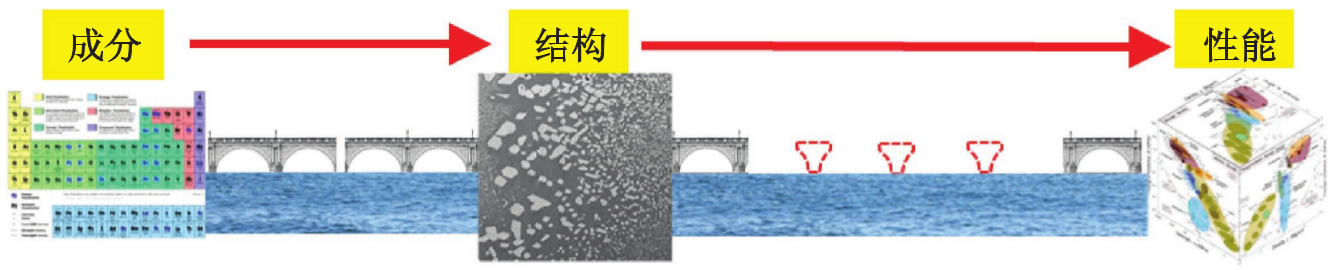
\includegraphics[height=0.80in,width=4.05in]{Figures/MGE-2.png}
%\caption{\tiny \textrm{Pseudopotential for metallic sodium, based on the empty core model and screened by the Thomas-Fermi dielectric function.}}%(与文献\cite{EPJB33-47_2003}图1对比)
\label{MGE}
\end{figure}
\begin{minipage}[c]{0.30\textwidth}
\begin{itemize}%[+-| alert@+>]
\vspace*{-2.25in}
 {\fontsize{7.5pt}{6.0pt}\selectfont
	 \setlength{\itemsep}{10pt}
 \item 变革研发模式,计算-实验-理论-数据科学相融合: 高效、低耗按需设计
 \item 数据驱动的材料创新平台主要面向复杂材料的模拟}
 \end{itemize}
\end{minipage}
\hfill
\begin{minipage}[b]{0.68\textwidth}
\begin{figure}[h!]
%\vspace*{-0.25in}
\centering
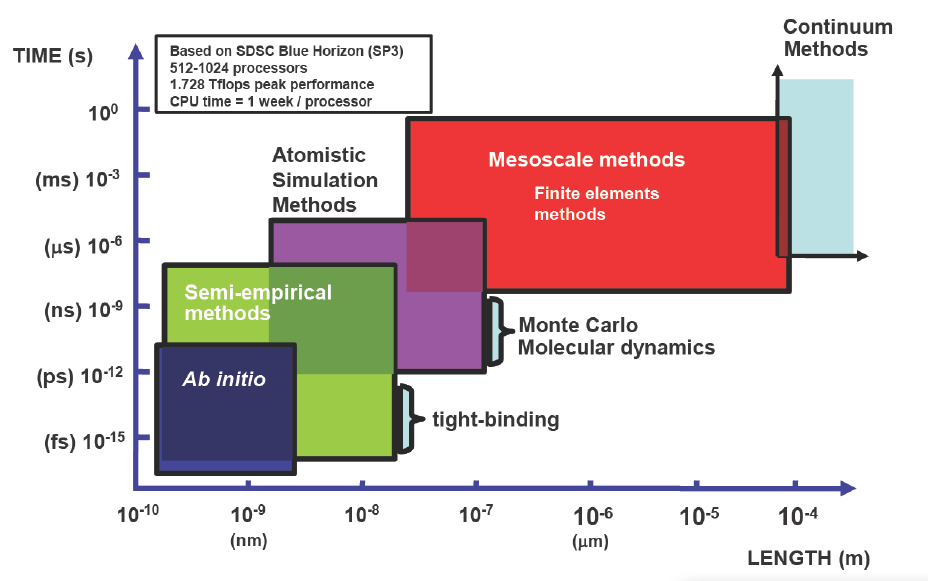
\includegraphics[height=1.80in,width=2.75in]{Figures/Multi-Scale-6.png}
%\caption{\tiny \textrm{Pseudopotential for metallic sodium, based on the empty core model and screened by the Thomas-Fermi dielectric function.}}%(与文献\cite{EPJB33-47_2003}图1对比)
\label{Multi-Scale}
\end{figure}
\end{minipage}
}

\frame
{
	\frametitle{科学研究的范式变更}
\begin{figure}[h!]
\vspace*{-0.28in}
\centering
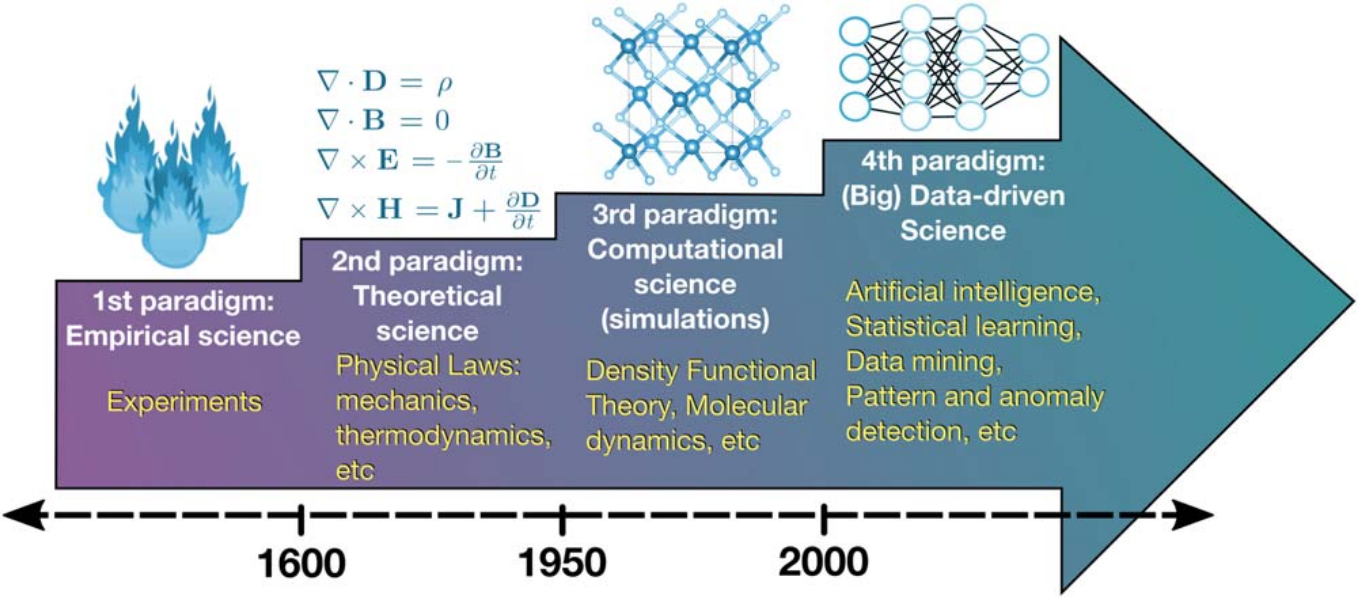
\includegraphics[height=2.00in,width=4.15in]{Figures/Four_Model_3.png}
%\caption{\tiny \textrm{Pseudopotential for metallic sodium, based on the empty core model and screened by the Thomas-Fermi dielectric function.}}%(与文献\cite{EPJB33-47_2003}图1对比)
\label{Four_Model}
\end{figure}
\begin{minipage}[b]{0.48\textwidth}
 {\fontsize{7.5pt}{6.0pt}\selectfont\begin{itemize}%[+-| alert@+>]
	 \setlength{\itemsep}{10pt}
 \item 逐步趋于理性
 \item 逐步趋于复杂
 \end{itemize}}
\end{minipage}
\hfill
\begin{minipage}[b]{0.48\textwidth}
 {\fontsize{7.5pt}{6.0pt}\selectfont\begin{itemize}%[+-| alert@+>]
	 \setlength{\itemsep}{10pt}
 \item 逐步趋于抽象
 \item 逐步趋于深刻
 \end{itemize}}
\end{minipage}
}

\frame
{
	\frametitle{数据驱动的科学研究}
前所未有的计算能力和大规模的数据收集能力%,现代科学正在进入“第四范式”:
\begin{figure}[h!]
%\vspace*{-0.05in}
\centering
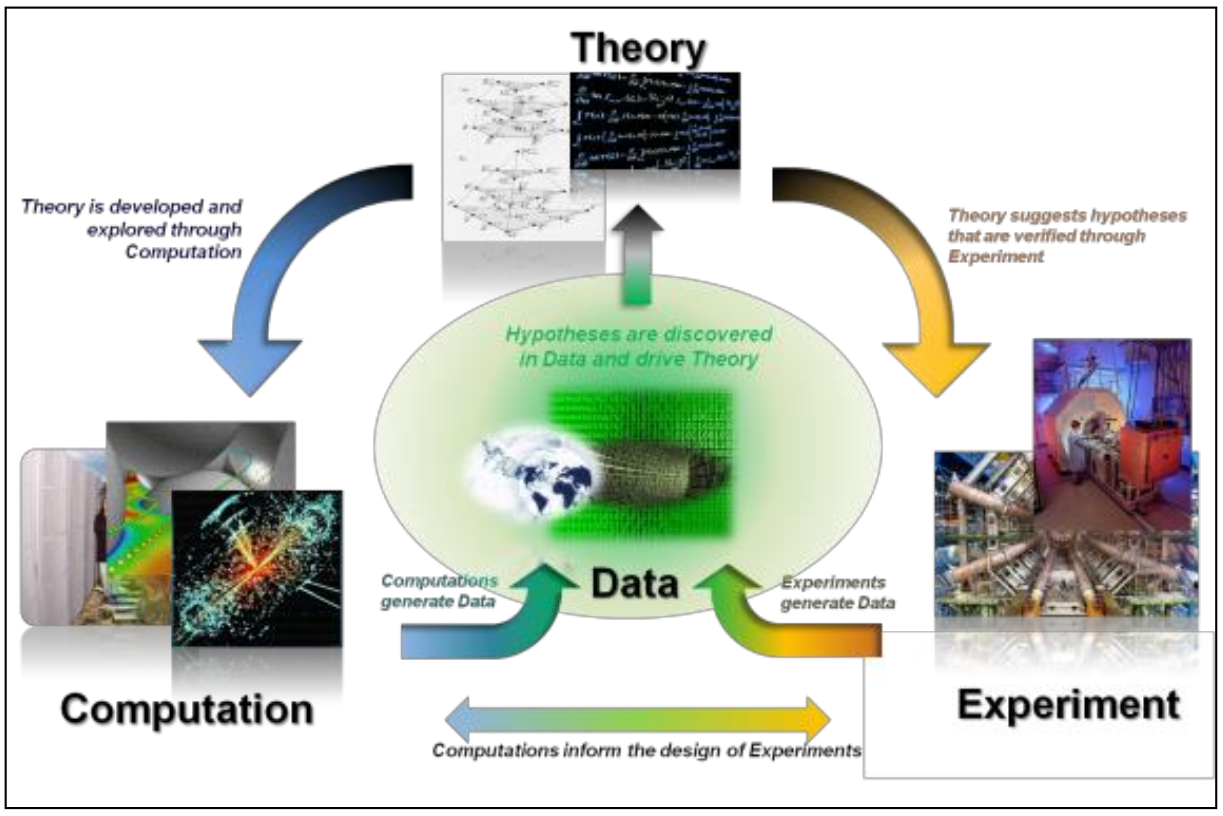
\includegraphics[height=2.30in,width=3.70in]{Figures/Four_Model_1.png}
%\caption{\tiny \textrm{Pseudopotential for metallic sodium, based on the empty core model and screened by the Thomas-Fermi dielectric function.}}%(与文献\cite{EPJB33-47_2003}图1对比)
\label{Four_Model_1}
\end{figure}
科学的新驱动力:~\textcolor{red}{密集数据}+\textcolor{red}{人工智能}\\
}

%\begin{frame}
%	\frametitle{理论、方法与软件}
%\begin{figure}[h!]
%\vspace*{-0.25in}
%\centering
%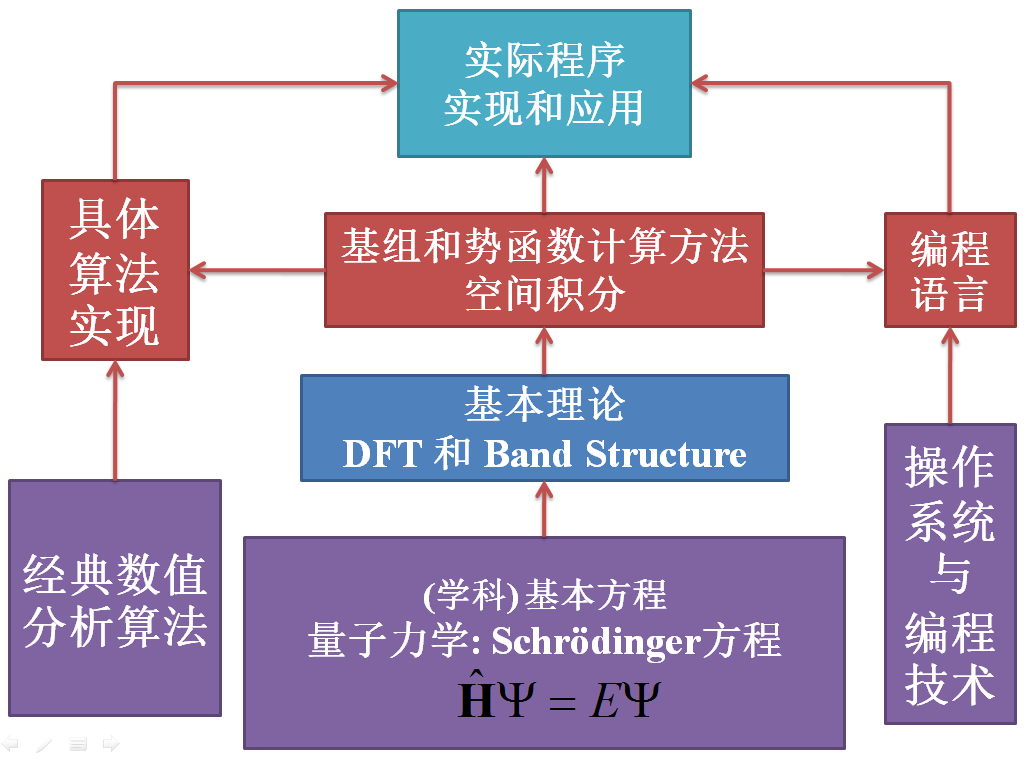
\includegraphics[height=2.80in,width=4.95in,viewport=5 3 1250 780,clip]{Figures/Method_Procedure.png}
%%\caption{\tiny \textrm{Pseudopotential for metallic sodium, based on the empty core model and screened by the Thomas-Fermi dielectric function.}}%(与文献\cite{EPJB33-47_2003}图1对比)
%\label{Method-Procedure}
%\end{figure}
%\end{frame}

\begin{frame}
	\frametitle{适应异质界面催化模拟自动流程软件}
\begin{minipage}[c]{0.42\linewidth}
\begin{itemize}
\vspace*{-2.75in}
%	\item “标准化”对称性分析功能:~降低\textrm{DFT}的计算量
	\item \textcolor{blue}{前处理}:\\
		计算模型分析与预处理
%	\item \textcolor{magenta}{$\vec k\cdot\vec p$方法}:~提升电子计算的规模%,为\textrm{DFT-MD}计算提供基础
	\item \textcolor{blue}{计算流程设计与管理}:\\
		\begin{enumerate}
			\item 支持计算过程的模块化
			\item 支持高通量、跨尺度材料模拟
			\item 提供计算结果数据管理接口
		\end{enumerate}
	\item \textcolor{blue}{后处理}:\\
		结果数据的分析、挖掘与可视化展示
%	\item \textcolor{magenta}{机器学习}:~优化电子计算结果,获得\textrm{MD}尺度力场,\textrm{DFT-MD}耦合%,获得\textrm{MD}尺度下准确的多体相互作用的力场函数。
%	\item 设计合理完善的程序流程:~利用\textrm{MongoDB}支持的\textrm{FireWorks}计算流程管理%,由微观尺度\textrm{DFT}计算获得介观或宏观尺度的计算物性或者使不同尺度的计算结果更好地实现耦合自洽
\end{itemize}
\end{minipage}
\hskip 2pt
\begin{minipage}[b]{0.47\linewidth}
\begin{figure}[h!]
\centering
%\hskip -35pt
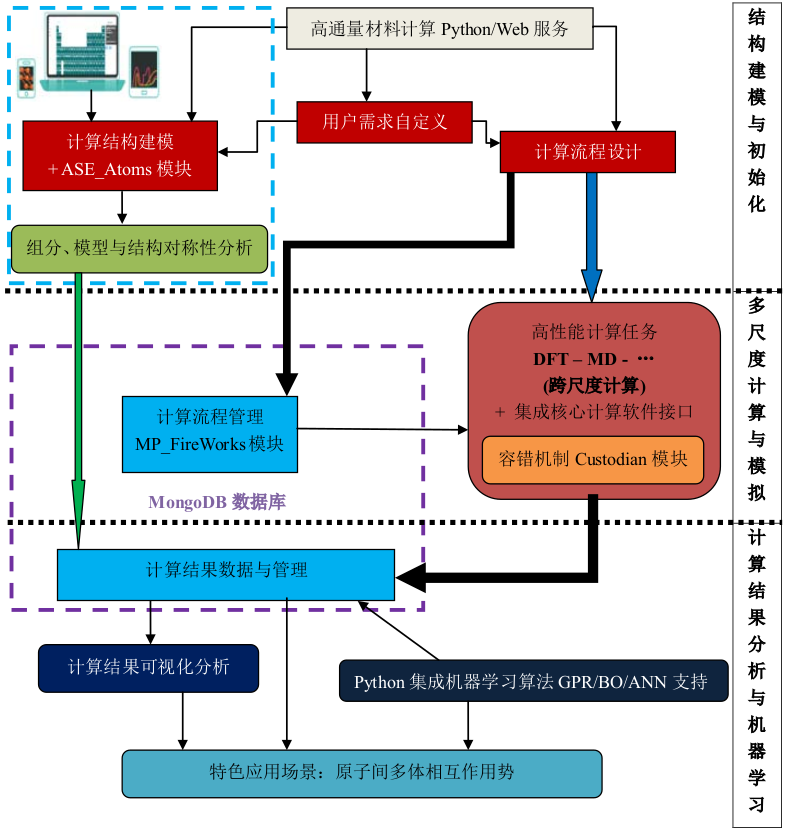
\includegraphics[height=2.18in]{Figures/MP_comp_BCC.png}
\caption{\fontsize{6.5pt}{4.5pt}\selectfont{适用于异质界面的高通量材料计算自动流程软件架构}}%
\label{MP_comp_BCC}
\end{figure}
\end{minipage}
\end{frame}

\begin{frame}
	\frametitle{材料智能计算平台}
	“\textcolor{magenta}{材料多尺度模拟仿真与多目标机器学习大数据平台}”
	\begin{itemize}
		\item 材料多尺度模拟流程,电子结构计算优化,化学反应动力学过程与多目标数据收集、特征工程、模型建立和验证等材料机器学习算法相融合
		\item 材料计算数据库技术应用:~晶体预测结构,半导体带隙,相稳定性,存能与功能材料的物理化学性质等
	\end{itemize}
\begin{figure}[h!]
\centering
\vspace*{-7pt}
%\animategraphics[autoplay, loop, width=3.95in, height=1.45in]{15}{Figures/DNN-}{0}{15}
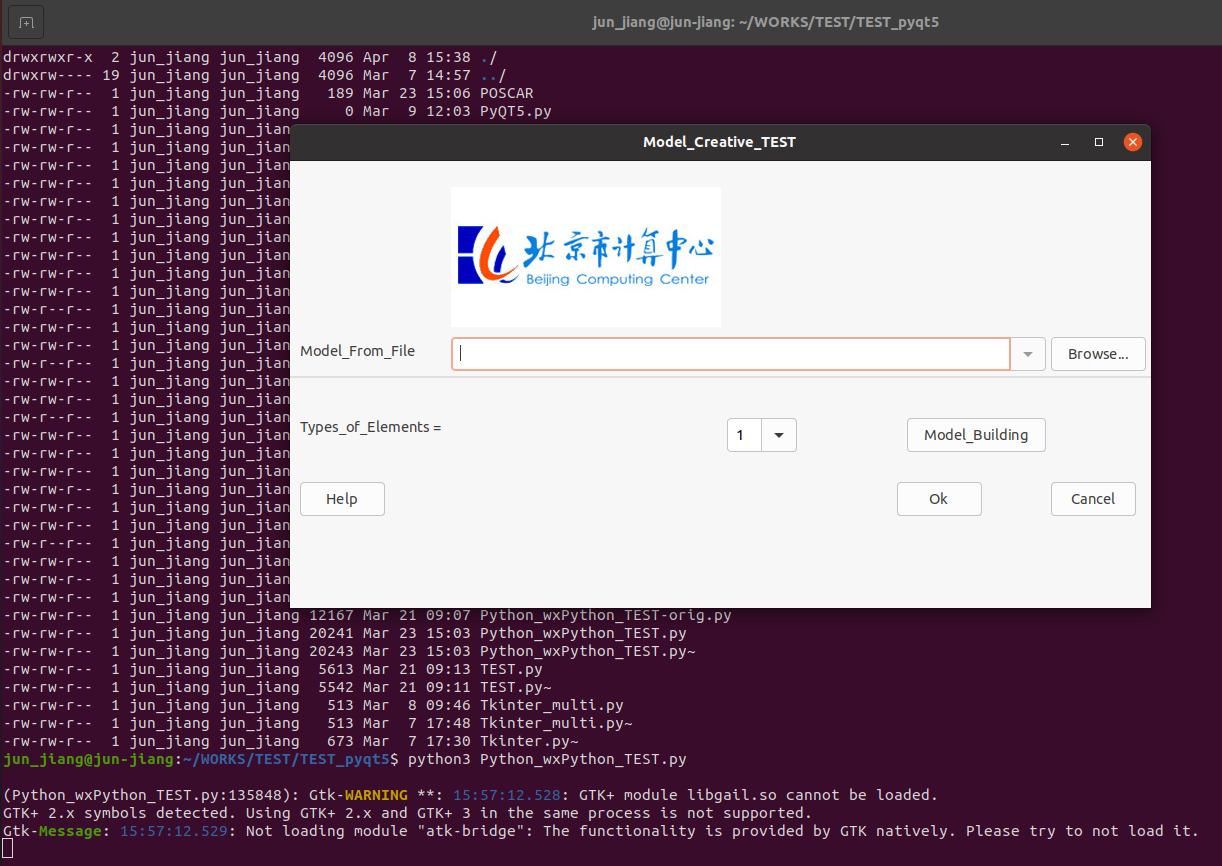
\includegraphics[height=1.60in,width=2.55in,viewport=0 0 1200 870,clip]{Figures/BCC-Process_1.png}
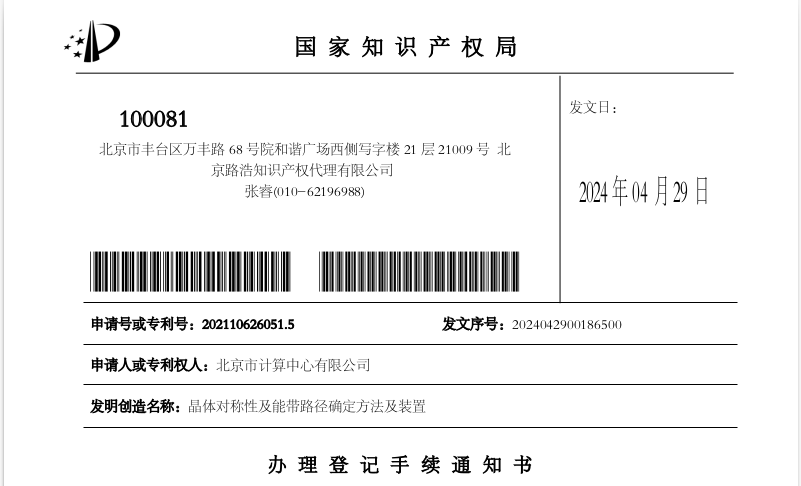
\includegraphics[height=0.85in,width=1.40in,viewport=0 0 801 486,clip]{Figures/Patent_license.png}
%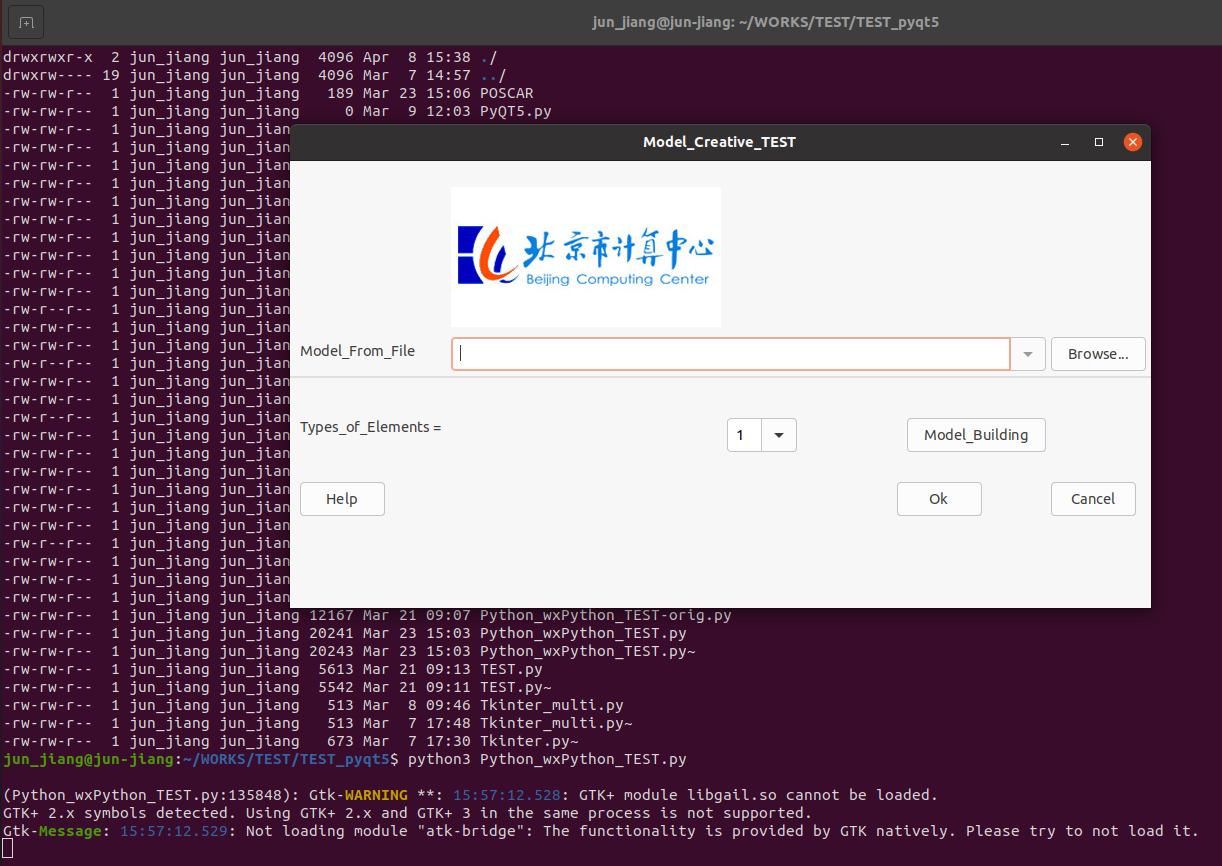
\includegraphics[height=2.00in,width=3.15in,viewport=0 0 1200 870,clip]{Figures/BCC-Process_1.png}
%\caption{\fontsize{6.5pt}{4.5pt}\selectfont{面向多尺度材料智能计算平台}}%
\label{BCC-Process_1}
\end{figure}
\end{frame}

\begin{frame}
	\frametitle{面向多尺度材料智能计算平台}
\begin{figure}[h!]
\centering
%\hskip -35pt
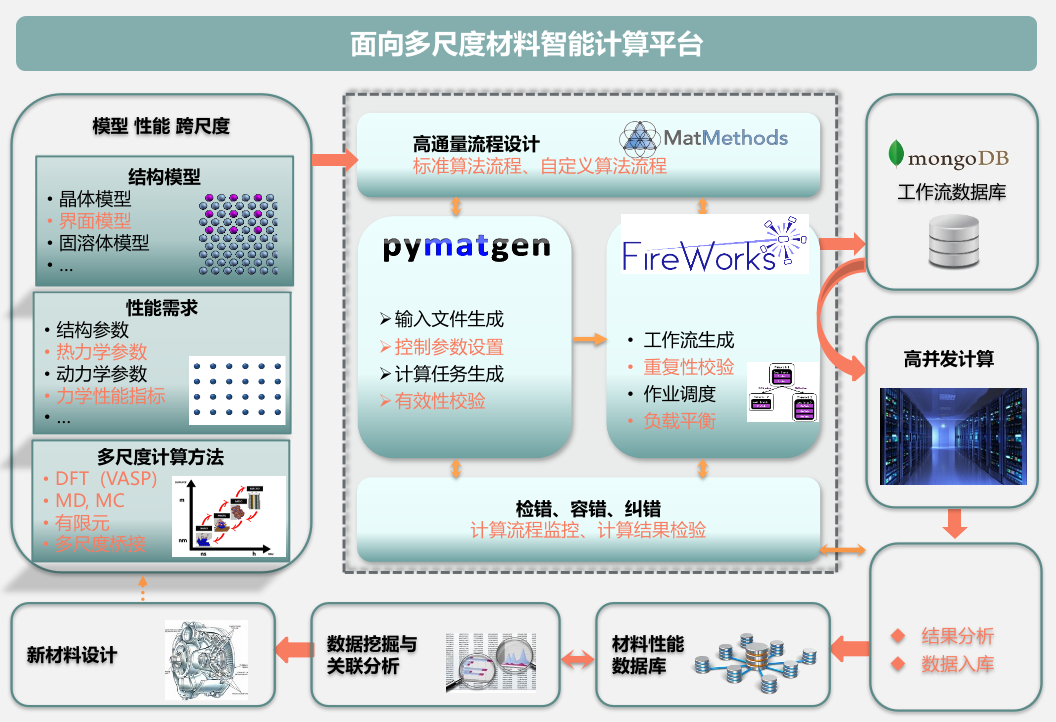
\includegraphics[height=2.75in]{Figures/MP_comp_BCC-2.png}
%\caption{\fontsize{6.5pt}{4.5pt}\selectfont{面向多尺度材料智能计算平台}}%
\label{MP_comp_BCC_2}
\end{figure}
\end{frame}

\begin{frame}
	\frametitle{应用:~类石墨烯材料产氢性能优化预测}
\begin{figure}[h!]
\centering
%\hskip -35pt
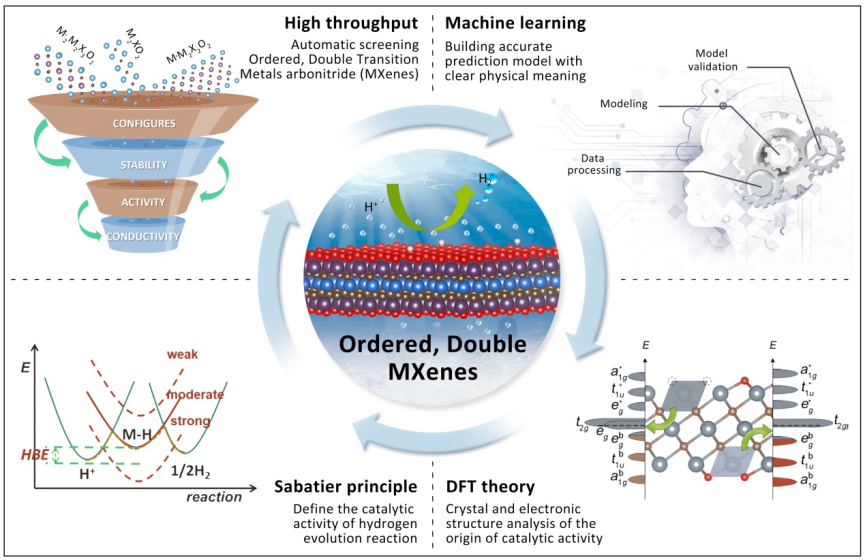
\includegraphics[height=1.85in]{Figures/MP_comp_BCC-3.png}
%\caption{\fontsize{6.5pt}{4.5pt}\selectfont{面向多尺度材料智能计算平台}}%
\label{MP_comp_BCC_3}
\end{figure}
{\fontsize{7.5pt}{5.5pt}\selectfont{
	应用高通量\textrm{DFT}计算,集成机器学习框架,预测\textrm{2D~MXenes}有序二元合金\textrm{(OBAs)}催化活性趋势并指导\textrm{HER}催化剂设计:}}
{\fontsize{5.5pt}{4.5pt}\selectfont{
	\begin{itemize}
		\item 由\textcolor{red}{数千个}\textrm{2D~MXenes}中筛选出的\textcolor{red}{110种}热稳定性、\textrm{HER}活性优于贵金属%\ch{Pt}
		\textrm{Pt}的潜在\textrm{2D~MXenes~OBAs}
	\item 特别是%\ch{Ti}
		\textrm{Ti}元素主要存在于\textrm{2D~MXenes~OBAs}理想催化剂中与实验合成的\textrm{MXenes}一致,\textcolor{red}{提高效率80\%}\\
	\end{itemize}
		获“\textcolor{blue}{2019中国大数据与智能计算技术创新奖}” \\
\textrm{J.~Mater.~Chem.~A,~2020} ~~~~~~~\url{https://doi.org/10.1039/D0TA06583H}}}
\end{frame}

\begin{frame}
	\frametitle{应用:~机器学习构建催化描述符}
\begin{figure}[h!]
\centering
%\hskip -35pt
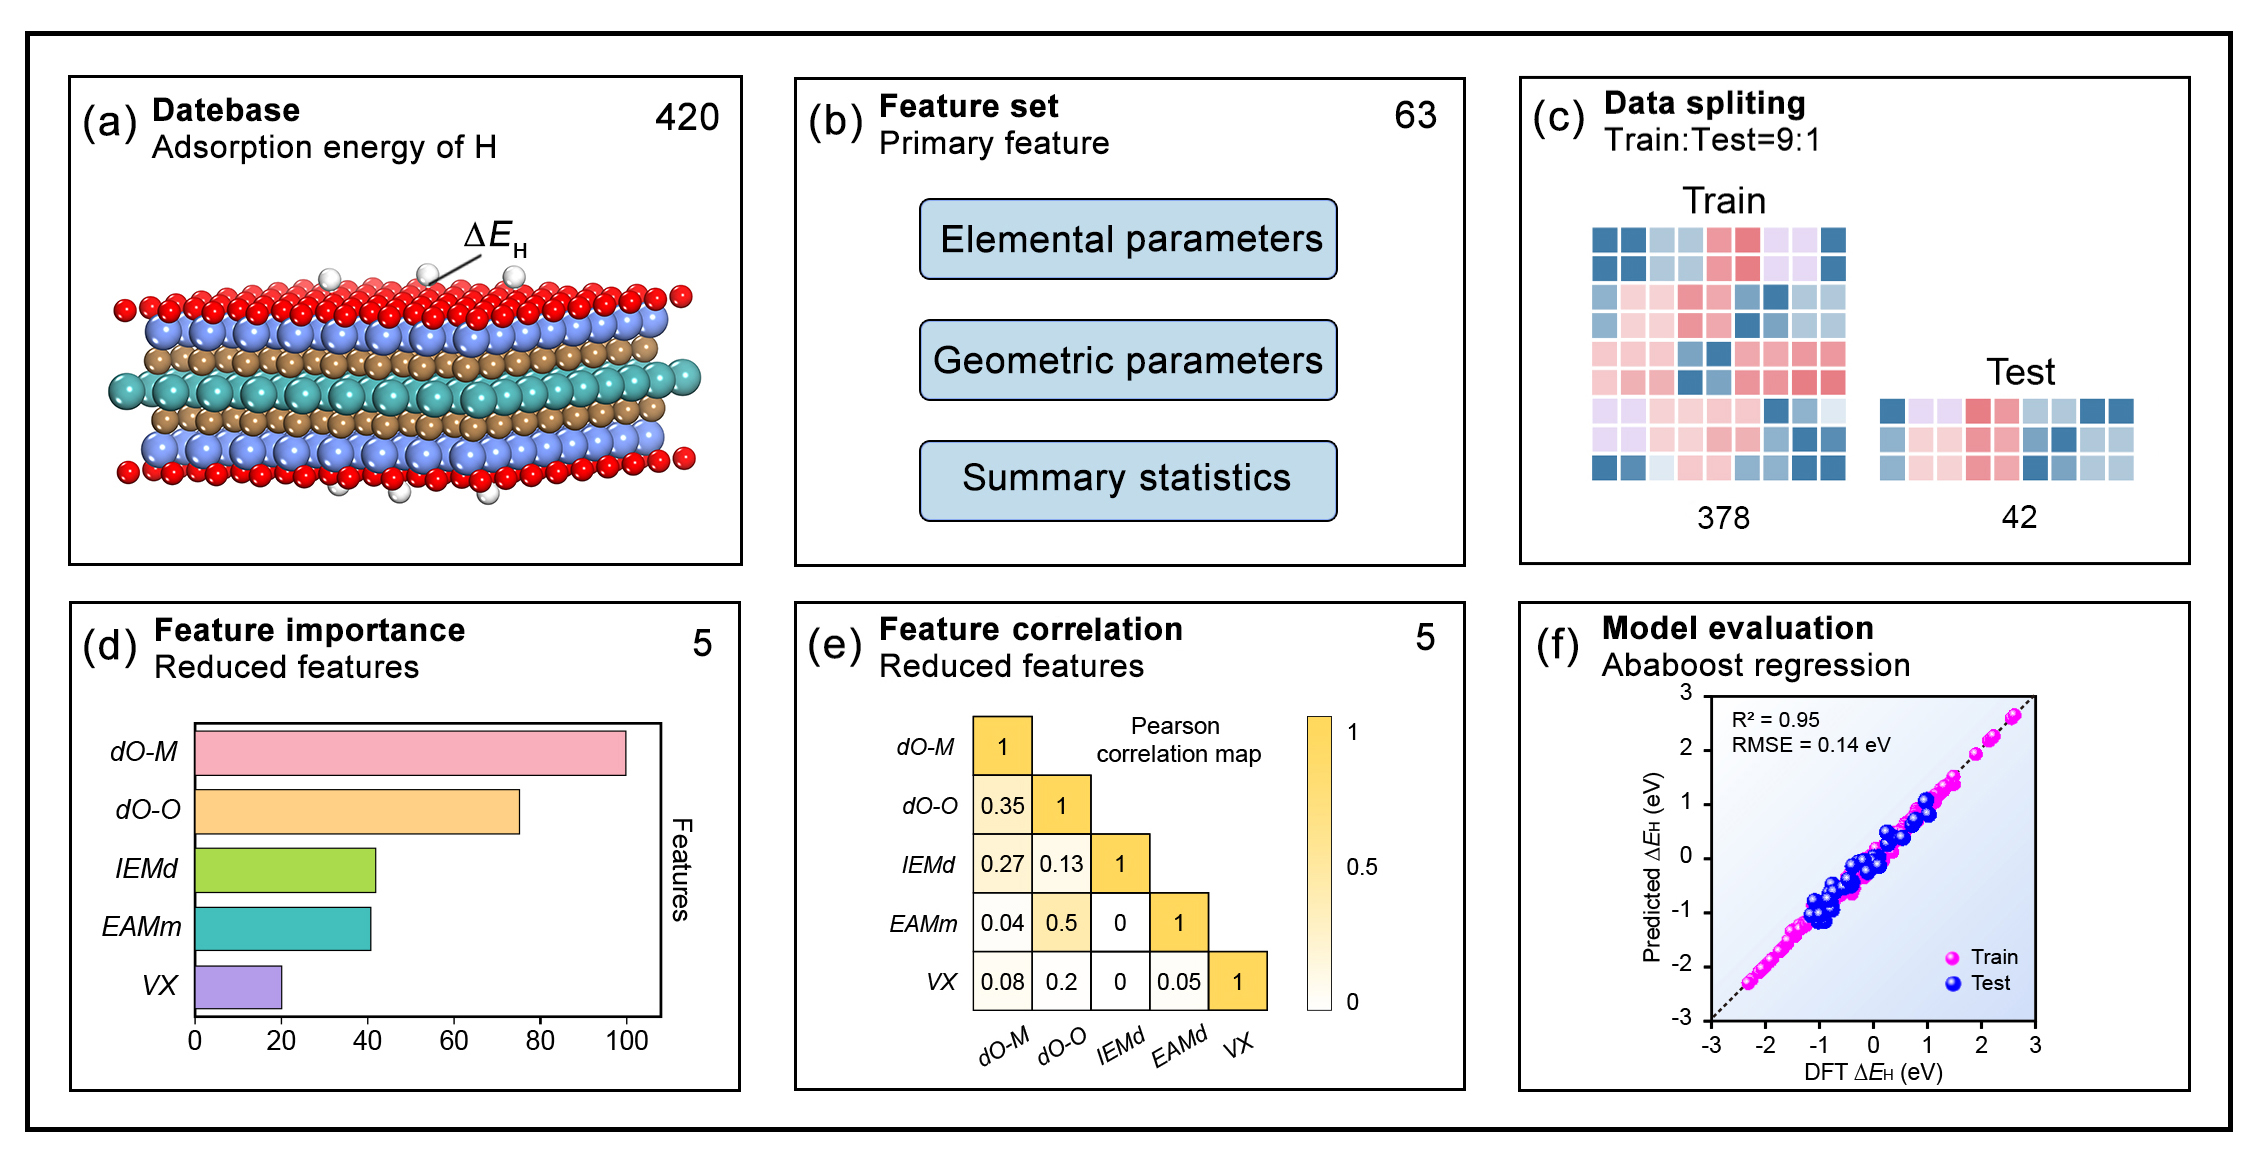
\includegraphics[height=1.85in]{Figures/MP_comp_BCC-4.png}
%\caption{\fontsize{6.5pt}{4.5pt}\selectfont{面向多尺度材料智能计算平台}}%
\label{MP_comp_BCC_4}
\end{figure}
{\fontsize{7.5pt}{5.5pt}\selectfont{
	面向\textrm{2D~MXenes}有序二元合金\textrm{(OBAs)}催化活性:
	\begin{itemize}
		\item 根据理化知识筛选特征向量
		\item 基于机器学习得到好的特征向量
		\item 对多目标优化,检验特征向量间相关度
		\item 基于特征向量筛选潜在优势催化活性材料
	\end{itemize}}}
\end{frame}

%\begin{frame}
%	\frametitle{应用:~类石墨烯材料的稳定性优化预测}
%\begin{figure}[h!]
%\centering
%%\hskip -35pt
%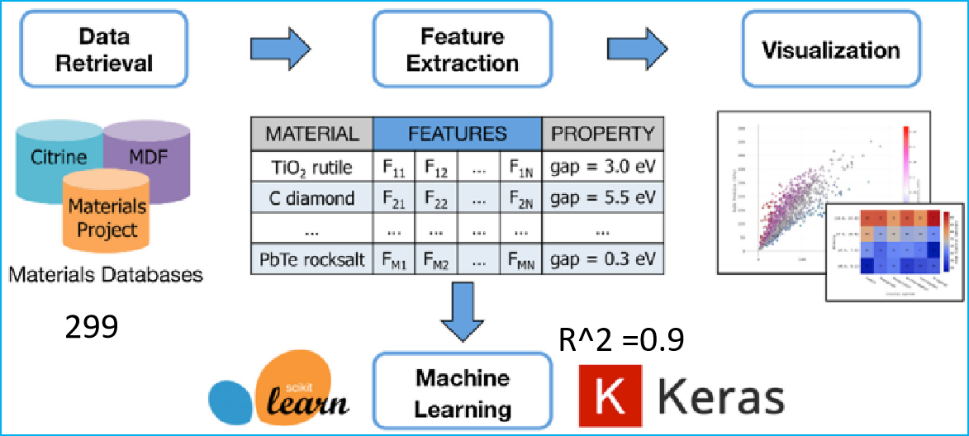
\includegraphics[height=1.55in]{Figures/MP_comp_BCC-5.png}
%%\caption{\fontsize{6.5pt}{4.5pt}\selectfont{面向多尺度材料智能计算平台}}%
%\label{MP_comp_BCC_5}
%\end{figure}
%{\fontsize{7.5pt}{5.5pt}\selectfont{
%	\begin{itemize}
%		\item 应用高通量建模软件构建潜在构型5600多种,利用\textrm{Materials~Projects}材料计算数据库提取竞争相数据
%		\item 通过热分解过程,组合化学反应式2000多组,筛选出热力学稳定的材料299种
%		\item 通过支持向量、高斯过程、随机深林、神经网络以及\textrm{adaboost}多种机器学习回归模型,利用13种常见特征参数对稳定性做了预测
%		\item 预测准确率达到94\%,节省计算成本高达70\%
%	\end{itemize}}}
%\end{frame}
%
%\begin{frame}
%	\frametitle{应用:~监督学习预测半导体材料带隙}
%\begin{figure}[h!]
%\centering
%\hspace*{-8pt}
%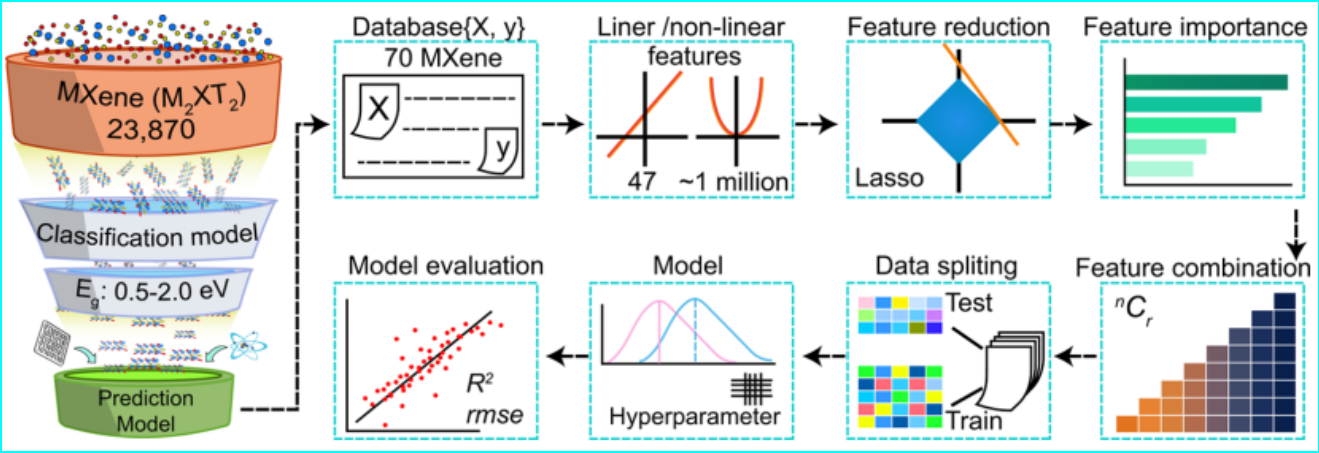
\includegraphics[height=1.45in]{Figures/MP_comp_BCC-6.png}
%%\caption{\fontsize{6.5pt}{4.5pt}\selectfont{面向多尺度材料智能计算平台}}%
%\label{MP_comp_BCC_6}
%\end{figure}
%{\fontsize{7.5pt}{5.5pt}\selectfont{
%	\begin{itemize}
%		\item 常规通行的材料模拟中带隙计算相当耗时
%		\item 利用%类石墨烯新能源
%	材料高通量智能计算与多目标机器学习集成研发平台,高通量自动化快速构建类石墨烯材料结构23870种,并构建数据库结合\textrm{KRR}、\textrm{SVR}、\textrm{GPR}、\textrm{Bagging}机器学习回归模型进行训练预测
%		\item \textrm{GPR}方法预测准确性达到了97\%,可以节省计算成本90\%多
%	\end{itemize}}}
%\end{frame}

\begin{frame}
	\frametitle{软硬件全方位集成}
	从自动流程到五阶数据创新材料软硬件一体机
\begin{figure}[h!]
\centering
%\hspace*{-8pt}
\includegraphics[height=1.75in]{Figures/BCC-5-steps_small.jpg}
%\includegraphics[height=1.45in]{Figures/BCC-5-steps.jpg}
%\caption{\fontsize{6.5pt}{4.5pt}\selectfont{面向多尺度材料智能计算平台}}%
\label{BCC-5-steps}
\end{figure}
%{\fontsize{7.5pt}{5.5pt}\selectfont{
\begin{itemize}
	\item 由材料模拟的物理规律转向数据处理能力的提升
	\item 五阶数据处理: 收集、分析、归档、清洗和标准化
	\item 探索数据认知能力,助力材料研究
\end{itemize}
\end{frame}

\begin{frame}[allowframebreaks]
	\frametitle{主要合作与推广应用}
		中科合成油(合作)
	\begin{itemize}
	 \setlength{\itemsep}{30pt}
	\item 化学-化工知识图谱的建设
\begin{figure}[h!]
\centering
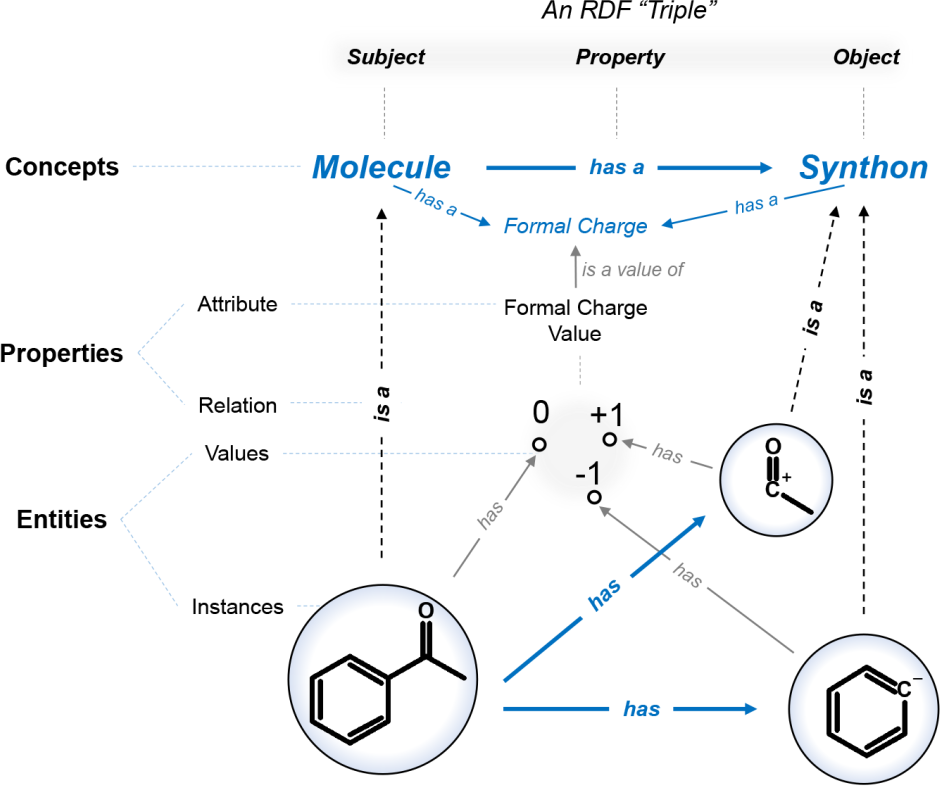
\includegraphics[height=1.50in,width=1.75in,viewport=0 0 950 790,clip]{Figures/Mapping-the-relationship-between-molecule-and-synthon.png}
\hspace{5pt}
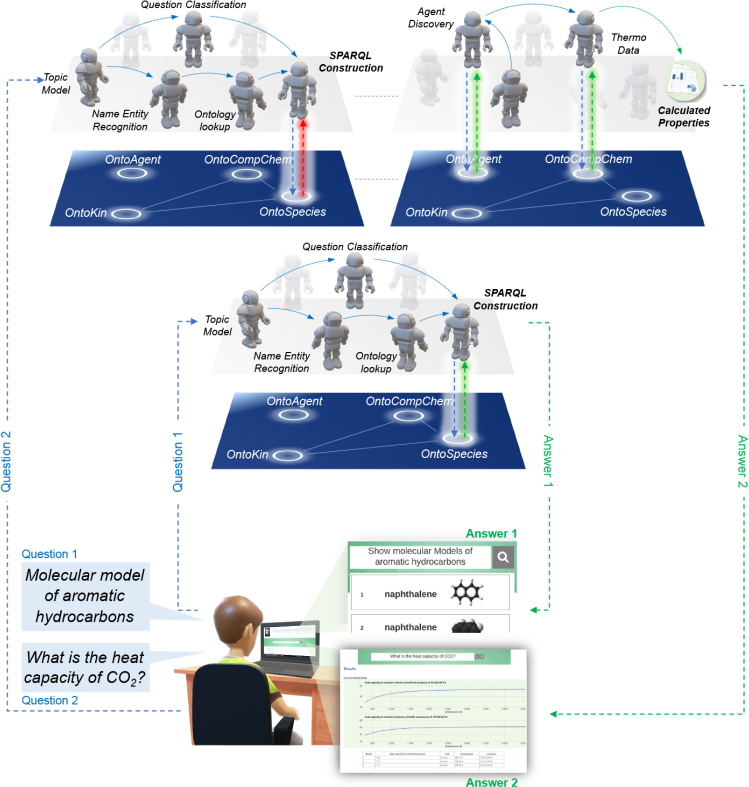
\includegraphics[height=1.50in,width=1.55in,viewport=0 0 750 790,clip]{Figures/TWA-KG-Marie.png}
%\caption{\small\textrm{Mapping the relationship molecule (chemical) and synthon (abstract) concepts and illustrating them with instrances. cite from\cite{ACR56-128_2023}}}%(与文献\cite{EPJB33-47_2003}图1对比)
\label{Fig:Mapping-relationship-molecule-synthon}
\end{figure}
	\begin{itemize}
{\fontsize{7.5pt}{5.5pt}\selectfont{
		\item 以化合物为核心,借助语义网\textrm{(Semantic Web)},组织、表示和存储化学-化工和领域特定类型的知识
		\item 构建拥有学习和推理能力,具备初级的创造知识的能力}}
	\end{itemize}
	\item 问-答式煤化工智能模型建设
\begin{figure}[h!]
\centering
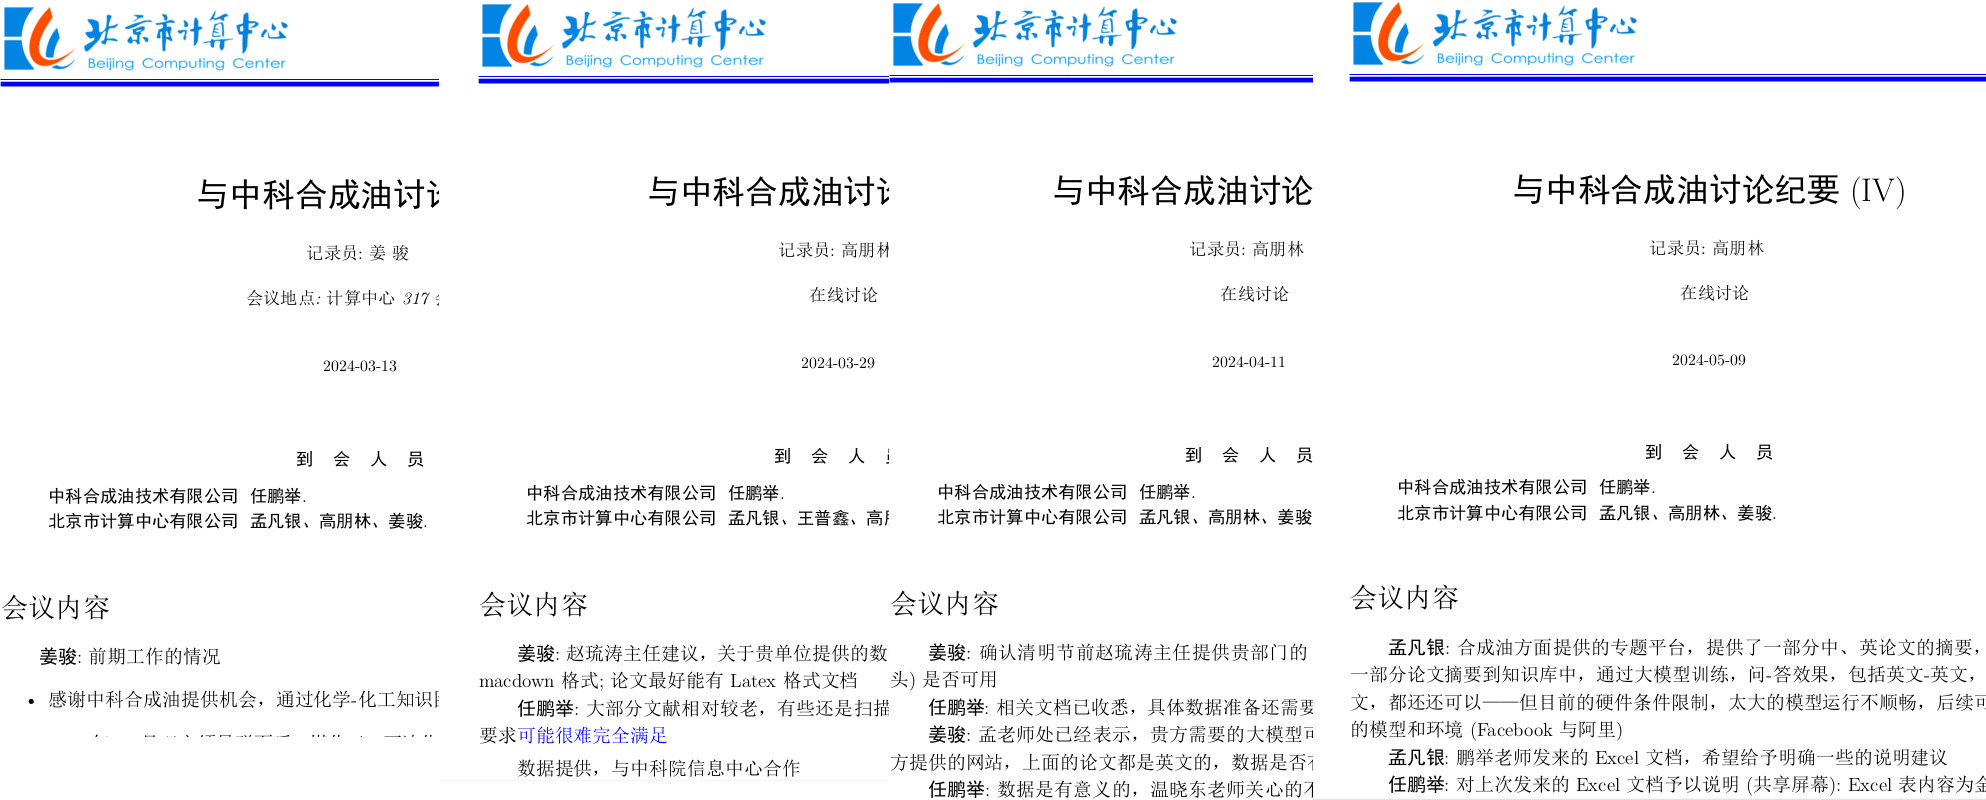
\includegraphics[height=1.40in,width=3.50in,viewport=0 0 1986 800,clip]{Figures/MeetingRecord_SCTC-BCC.png}
\label{Fig:Meeting_Record}
\end{figure}
\begin{itemize}
	\item 面向人工智能的全方位转型:\\
		面向碳基础材料、发挥人工智能的作用
	\item 大模型加持专业知识
\end{itemize}
	\end{itemize}
\textcolor{purple}{目标:}~智能实验室-智能科学家
\end{frame}

\begin{frame}
	\frametitle{主要合作与推广应用}
中科院物理所(推广)
	\begin{itemize}
	 \setlength{\itemsep}{10pt}
		\item 提供的流程软硬件一体机支持凝聚态物理的理论研究
		\item 深化对拓扑绝缘体材料物性特征的认知%,加速对潜在拓扑绝缘体材料的发现
\begin{figure}[h!]
\centering
\vskip 5pt
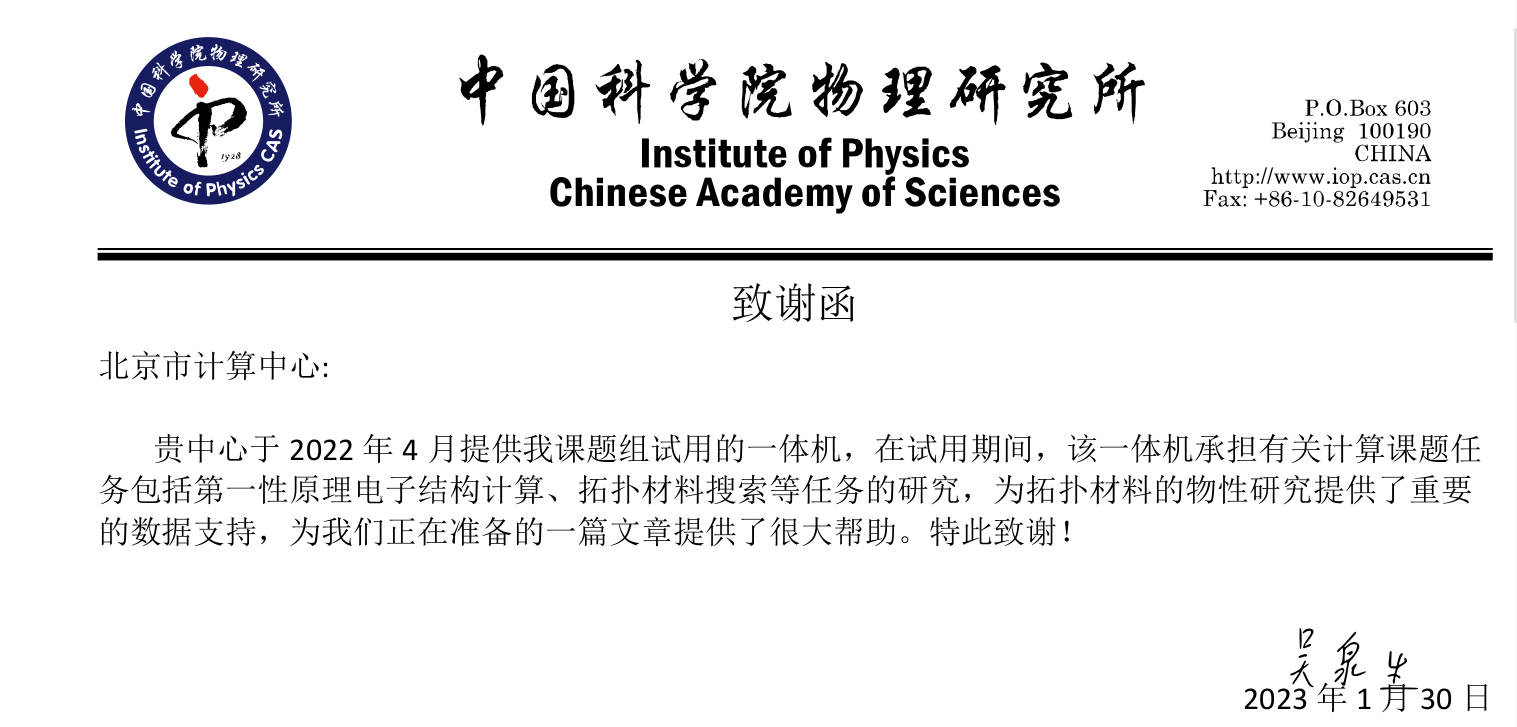
\includegraphics[height=1.7in]{Figures/Acknowledge-IP_CAS-BCC.png}
%\caption{\fontsize{6.5pt}{4.5pt}\selectfont{面向多尺度材料智能计算平台}}%
\label{Acknowleges-IP_CAS}
\end{figure}
	\end{itemize}
\end{frame}

\begin{frame}
	\frametitle{数据驱动的材料研发:~应用前景}
	\begin{enumerate}
	 \setlength{\itemsep}{20pt}
	 \item 航空发动机材料:~\textcolor{blue}{镍基单晶高温合金材料}\\
	合金组分优化与强化功能提升

\item 煤化工催化材料:~\textcolor{blue}{新型铁触媒材料}\\
	反应活化性能提升与化学平衡的移动

		\item 稀土功能材料:~\textcolor{blue}{钕铁硼永磁材料},\textcolor{blue}{稀土发光材料}\\
	3\textit{d}-4\textit{f} 电子相互作用机制的认知

	\end{enumerate}

	\textcolor{magenta}{材料组分趋于复杂、材料机理认知趋于微观、材料与数据趋于膨胀}
%\begin{figure}[h!]
%\vspace*{-0.20in}
%\centering
%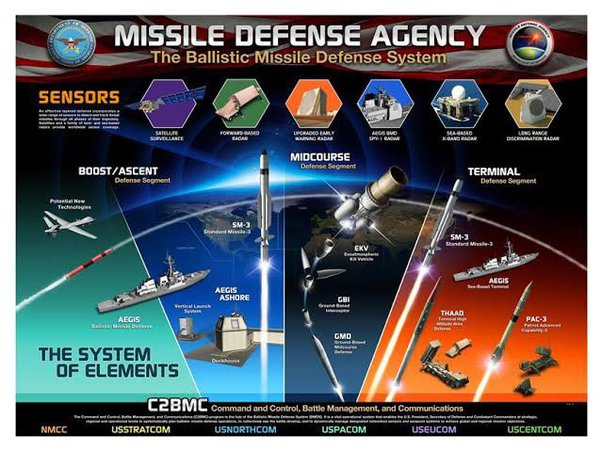
\includegraphics[height=2.90in,width=3.70in]{Figures/Main-qimg.jpeg}
%\label{BMDS}
%\end{figure}
\end{frame}
%------------------------------------------------------------------------Reference----------------------------------------------------------------------------------------------
%		\frame[allowframebreaks]
%{
%\frametitle{主要参考文献}
%\begin{thebibliography}{99}
%{\tiny
%	\bibitem{PR136-B864_1964}\textrm{P. Hohenberg and W. Kohn, \textit{Phys. Rev.} \textbf{136} (1964), B864}
%	\bibitem{PR140-A1133_1965}\textrm{W. Kohn and L.J. Sham, \textit{Phys. Rev.} \textbf{140} (1965), A1133}
%	\bibitem{PRB50-17953_1994}\textrm{P. E. Bl\"ochl. \textit{Phys. Rev.} B, \textbf{50} (1994), 17953}
%	\bibitem{PRB59-1758_1999}\textrm{G. Kresse and D. Joubert \textit{Phys. Rev.} B, \textbf{59} (1999), 1758}
%	\bibitem{Elect_Stru}\textrm{Richard. M. Martin. \textit{Electronic Structure: Basic Theory and Practical Methods} (Cambridge University Press, Cambridge, England, 2004)}
%        \bibitem{Singh}\textrm{D. J. Singh. \textit{Plane Wave, PseudoPotential and the LAPW method} (Kluwer Academic, Boston,USA, 1994)}					%
%}
%\end{thebibliography}
%%\nocite*{}
%}
%-----------------------------------------------------------------------------------------------------------------------------------------------------------------------%
